%!TEX program = lualatex

\documentclass[17pt]{beamer} % notes, notes=only
%\documentclass[handout]{beamer}
%\documentclass[aspectratio=169]{beamer}

\usetheme{EastLansing}
\usecolortheme{seagull}
\useinnertheme{rectangles}
\usefonttheme{professionalfonts}

\usepackage[utf8]{inputenc}
\usepackage[T1]{fontenc}
\usepackage[ngerman]{babel}

\usepackage{libertine}
%\usepackage{microtype}

\setmainfont[Ligatures=TeX]{Linux Biolinum O}
%\setmathfont[math-style=ISO,bold-style=ISO,vargreek-shape=TeX,Ligatures=TeX]{TeX Gyre Pagella Math}




\beamertemplatenavigationsymbolsempty
\AtBeginSection{\sectionpage}


\title[]{Willkommen zur Generalversammlung von FunkFeuer Wien}
%\author{}
%\institute[]{}
\subtitle[]{Eintreffen ab 18:00, Start der GV um 18:30}
\date[]{2020-05-19\\\tiny CC BY-SA 4.0}


\def\Put(#1,#2)#3{\leavevmode\makebox(0,0){\put(#1,#2){#3}}}

\newcommand\scaleheight{0.7}



\begin{document}


\frame{\titlepage}

%%%%%%%%%%%%%%%%%%%%%%%%%%%%%%%%%%%%%%%%%%%%%%%%%%%%%%%%%%%%%%%%%%%%%%%%
%
% \begin{frame}
% 	\frametitle{Outline}
% 	\tableofcontents
% \end{frame}
% \note[itemize] {
% 	\item NOTIZ HIER
% }

%%%%%%%%%%%%%%%%%%%%%%%%%%%%%%%%%%%%%%%%%%%%%%%%%%%%%%%%%%%%%%%%%%%%%%%%
\begin{frame}
	\frametitle{Begrüßung}
	Beginn der Generalversammlung um 18:30.
\end{frame}



%%%%%%%%%%%%%%%%%%%%%%%%%%%%%%%%%%%%%%%%%%%%%%%%%%%%%%%%%%%%%%%%%%%%%%%%
\begin{frame}
	\frametitle{Feststellen der Beschlussfähigkeit}
	nach §9 Abs. 6:
	\textit{,,Die Generalversammlung ist ohne Rücksicht auf die Anzahl der
	Erschienenen beschlussfähig.''}
\end{frame}



%%%%%%%%%%%%%%%%%%%%%%%%%%%%%%%%%%%%%%%%%%%%%%%%%%%%%%%%%%%%%%%%%%%%%%%%
\begin{frame}
	\frametitle{Was haben wir vor uns?}
	\begin{itemize}
		\item Berichte des Vorstands
		\item Abstimmung über Entlastung
		\item Wahlen: Vorstand, Rechnungsprüfung
		\item Abstimmungen über Anträge
		\item Allfälliges
	\end{itemize}
\end{frame}


%%%%%%%%%%%%%%%%%%%%%%%%%%%%%%%%%%%%%%%%%%%%%%%%%%%%%%%%%%%%%%%%%%%%%%%%
\begin{frame}{FunkFeuer}

Internet zum Mitmachen auf allen Ebenen

  \begin{figure}
    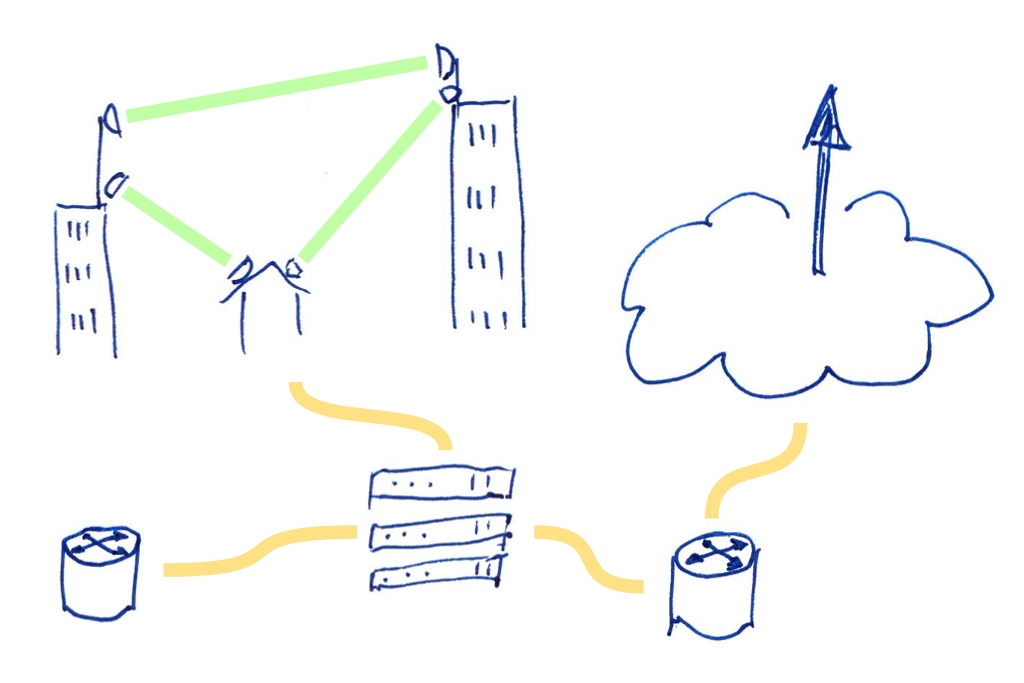
\includegraphics[width=0.8\textwidth]{figures/FunkFeuer_Ueberblick.jpg}
  \end{figure}
\end{frame}
\note[itemize]{
    \item Netzlayer (Dienste, Maschinen, Housing, Wartung, Linktechnologien, ...)
    \item Technisch, sozial, international
    \item Demokratisch
}


%%%%%%%%%%%%%%%%%%%%%%%%%%%%%%%%%%%%%%%%%%%%%%%%%%%%%%%%%%%%%%%%%%%%%%%%
\begin{frame}{FunkFeuer}
  \begin{figure}
    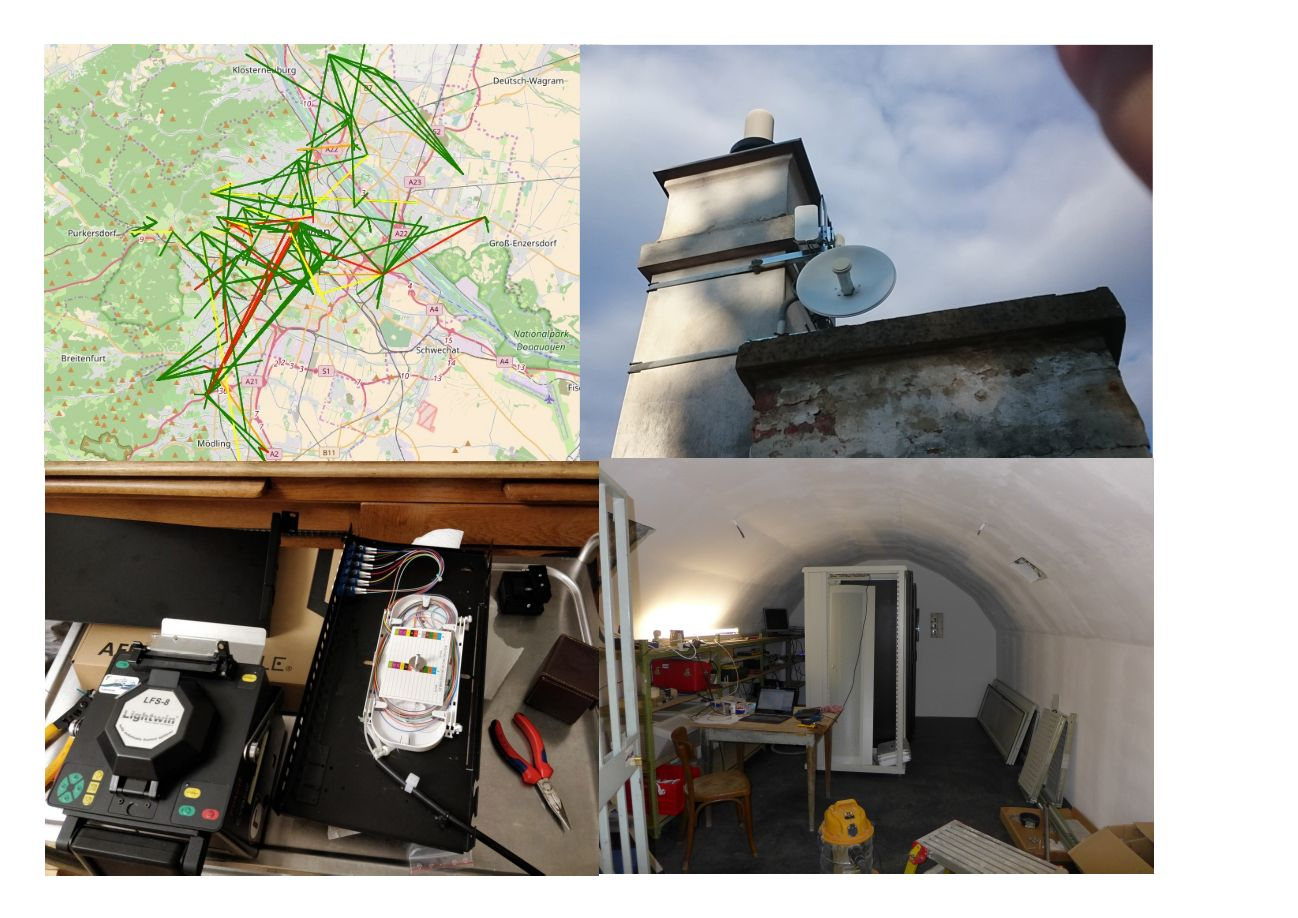
\includegraphics[width=0.85\textwidth]{figures/FunkFeuer_Bilder.jpg}
  \end{figure}
\end{frame}



%%%%%%%%%%%%%%%%%%%%%%%%%%%%%%%%%%%%%%%%%%%%%%%%%%%%%%%%%%%%%%%%%%%%%%%%
\begin{frame}
	\frametitle{Bericht des Vorstands}
	\begin{itemize}
		\item Regelmäßig wiederkehrende Aktivitäten
		\item ,,Außertourliche'' Aktivitäten
	\end{itemize}
\end{frame}
\note[itemize] {
	\item Mitgliedsverwaltung
	\item Housing-Verwaltung
	\item Bankeinzüge
	\item Rechnungen bezahlen, Refundierungen
	\item MoMos
	\item Behördenkontakt (LPD, FMB, RTR)
	\item Verträge verhandeln, abschließen, auflösen
}



%%%%%%%%%%%%%%%%%%%%%%%%%%%%%%%%%%%%%%%%%%%%%%%%%%%%%%%%%%%%%%%%%%%%%%%%
\begin{frame}
	\frametitle{Bericht des Vorstands}
	\begin{itemize}
		\item ,,MoMo'' -- monatliche Montagstreffen
		\item Fernmeldebehörde, Austro Control
		\item RTR
		\item Neues Housing
	\end{itemize}
\end{frame}
\note[itemize] {
	\item MoMos sind sehr gut besucht (5-20 Leute, alt/jung/neu/erfahren). Danke David für die Initiative!
	\item FMB: Funküberwachung meldete Störung des Wetter-RADARs am Flughafen Wien. Schnelles Handeln nötig, öffentliche Wirkung (auf Verein und Ministerium) gewünscht; 
}



%%%%%%%%%%%%%%%%%%%%%%%%%%%%%%%%%%%%%%%%%%%%%%%%%%%%%%%%%%%%%%%%%%%%%%%%
\begin{frame}
	\frametitle{Bericht des Kassiers (1/2)}
	\begin{itemize}
		\item Einnahmen knapp 2k€/Monat (Housing)
		\item Ausgaben für Strom, RIPE, ISPA, Uplink, Steuerberatung
		\item Investitionen: Hardware, Dark Fiber, Roofnode Anexia, 60-GHz-Bounty
		\item \textbf{402 € Spenden}
	\end{itemize}
\end{frame}



%%%%%%%%%%%%%%%%%%%%%%%%%%%%%%%%%%%%%%%%%%%%%%%%%%%%%%%%%%%%%%%%%%%%%%%%
\begin{frame}
	\frametitle{Bericht des Kassiers (2/2)}
	Umzug des Housings:
	\begin{itemize}
		\item Neuer Standort, weiterhin Bittleihe
		\item Bisherige Kosten knapp 11k€
		\item Noch keine Dark Fiber!
	\end{itemize}
\end{frame}
\note[itemize] {
	\item Status: fast fertig, einige Arbeit fehlt noch
	\item Ansparkonto für Dark Fiber wurde nicht angerührt
}



%%%%%%%%%%%%%%%%%%%%%%%%%%%%%%%%%%%%%%%%%%%%%%%%%%%%%%%%%%%%%%%%%%%%%%%%
\begin{frame}
	\frametitle{Bericht der Rechnungsprüfer}
\end{frame}



%%%%%%%%%%%%%%%%%%%%%%%%%%%%%%%%%%%%%%%%%%%%%%%%%%%%%%%%%%%%%%%%%%%%%%%%
\begin{frame}
	\frametitle{Kurze Pause}
	Um ....... Uhr geht es weiter mit der Entlastung des Vorstands und
	den Wahlen
\end{frame}



%%%%%%%%%%%%%%%%%%%%%%%%%%%%%%%%%%%%%%%%%%%%%%%%%%%%%%%%%%%%%%%%%%%%%%%%
\begin{frame}
	\frametitle{Abstimmung über Entlastung des Vorstands}
	(für den Anteil der Funktionsperiode im Geschäftsjahr)
\end{frame}
\note[itemize] {
	\item Das Geschäftsjahr des Vereins beginnt (generell) unabhängig und
	(momentan) nicht gleichzeitig mit der Funktionsperiode des Vorstands
	\item Eine Angleichung wurde bereits vorgeschlagen, aber abgelehnt
	\item \url{https://wiki.funkfeuer.at/wiki/Regionen/Wien/Verein/201805_GV_Protokoll\#Antrag_auf_Angleichung_des_Gesch.C3.A4ftsjahres}
}



%%%%%%%%%%%%%%%%%%%%%%%%%%%%%%%%%%%%%%%%%%%%%%%%%%%%%%%%%%%%%%%%%%%%%%%%
\begin{frame}
	\frametitle{Wahlen}
	\begin{itemize}
		\item Vorstellungsrunde der Kandidierenden
		\item Wahl der Vorstandsfunktionen
		\item Wahl der Rechnungsprüfer
		\item Annahme der Wahl
	\end{itemize}
\end{frame}



%%%%%%%%%%%%%%%%%%%%%%%%%%%%%%%%%%%%%%%%%%%%%%%%%%%%%%%%%%%%%%%%%%%%%%%%
\begin{frame}
	\frametitle{Kurze Pause}
	Um ....... Uhr geht es weiter mit Anträgen
\end{frame}



%%%%%%%%%%%%%%%%%%%%%%%%%%%%%%%%%%%%%%%%%%%%%%%%%%%%%%%%%%%%%%%%%%%%%%%%
\begin{frame}
	\frametitle{Anträge an die Generalversammlung}
\end{frame}



%%%%%%%%%%%%%%%%%%%%%%%%%%%%%%%%%%%%%%%%%%%%%%%%%%%%%%%%%%%%%%%%%%%%%%%%
\begin{frame}
	\frametitle{Anträge Änderung der Statuten}
	\url{https://gitlab.com/funkfeuer/Statuten-Wien/merge_requests}
\end{frame}



%%%%%%%%%%%%%%%%%%%%%%%%%%%%%%%%%%%%%%%%%%%%%%%%%%%%%%%%%%%%%%%%%%%%%%%%
\begin{frame}
	\frametitle{Allfälliges}
	\begin{itemize}
		\item ,,Neuhousing''-Projekt (Vortrag, 5 min)
		\item Weitere Wortmeldungen
	\end{itemize}
\end{frame}



%%%%%%%%%%%%%%%%%%%%%%%%%%%%%%%%%%%%%%%%%%%%%%%%%%%%%%%%%%%%%%%%%%%%%%%%
\begin{frame}
	\frametitle{Das war's}
	Danke für's Dabeisein!
\end{frame}

%%%%%%%%%%%%%%%%%%%%%%%%%%%%%%%%%%%%%%%%%%%%%%%%%%%%%%%%%%%%%%%%%%%%%%%%
\end{document}
